\section{Results}

\newcolumntype{C}[1]{>{\centering\let\newline\\\arraybackslash\hspace{0pt}}m{#1}}

\begin{table*}[]
\centering
\label{my-label}
\begin{tabular}{|c|C{0.8cm}|C{0.8cm}|C{0.8cm}|C{0.8cm}|C{0.8cm}|C{0.8cm}|C{0.8cm}|C{0.8cm}|C{0.8cm}|C{0.8cm}|C{0.8cm}|C{0.8cm}|}
\hline
\multirow{2}{*}{Motion} & \multicolumn{2}{c|}{Ours} & \multicolumn{2}{c|}{Joint Position} & \multicolumn{2}{c|}{Yaw Pitch Roll} & \multicolumn{2}{c|}{Quaternion} & \multicolumn{2}{c|}{Matrix Elements} & \multicolumn{2}{c|}{$\mathfrak{se}3$ only} \\ \cline{2-13} 
                        &$t$ &$e$  &$t$  &$e$  &$t$  &$e$  &$t$  &$e$  &$t$  &$e$  &$t$  &$e$  \\ \hline
Dunk(90 frames)         &3.18 &9.88   &2.14 &40.71    &6.544 &55.38  &3.88 &10.03  &4.01 &11.15    &3.04 &12.73 \\ \hline
Walk(397 frames)        &1.78 &4.48   &1.60 &13.48    &11.70 &36.60     &4.55 &21.35  &2.63 &15.26    &1.72 &4.96 \\ \hline
Jump*(90 frames)     &3.52 &20.30   &3.67 &56.41   &8.17 &51.36  &4.20 &28.61  &2.32 &26.18       &4.33 &41.73 \\ \hline
Average			     &2.83 &11.55   &2.47 &36.87   &8.80 &47.78      &4.21 &20.00  &2.99 &17.53   &3.03 &19.81 \\ \hline
\end{tabular}
\caption{Average error $e$ and comutation time $t$ required for the mapping of three different target motions using various skeletal representations.
The character has 85 rig space parameters and 35 skeletal segments, and we limit the maximum iteration to 100.
$e$ is calculated in the proposed skeletal representation, and the unit of $t$ is $sec/frame$.
*Jump motion includes stylized squash-and-stretch motion as shown in Figure~\ref{fig:squashResult}.
}
\label{table:poseRepresentEvaluation}
\end{table*}

We first compare the proposed skeletal pose representation with other representations. Next, we present several examples to demonstrate how our optimization resolves ambiguity caused by the inverse mapping and modifies the results corresponding to the input by the artist. We applied our method to the animation production pipeline to verify that our method can actually improve the productivity in the creation and editing of character animation in the real production environment.

To verify the versatility of our motion mapping, we performed the experiments with various characters.
Both motion capture data and keyframed animations were used as retargeting sources, and all the motions were adjusted to be 30 frames per second. To test our method in the Autodesk Maya 2016 environment, we implemented the system as a plug-in with Maya python script. A 3.40GHz Intel i7-3770 processor with 8GB memory is utilized for all of the experiments.

\textbf{Pose representation evaluation}
We performed the same rig space motion mapping with different skeletal representations to show that the proposed skeletal representation outperforms the other representations in terms of efficiency and correctness. We measured the computation time and the error of the skeleton at joint positions, joint angles(Yaw-Pitch-Roll), Quaternion, elements of a transformation matrix, hierarchy only representation of Lie group, and our representation. Table~\ref{table:poseRepresentEvaluation} shows the results. The result verfies that our pose representation provides an efficient and precise solution compared to other pose representations.

\textbf{Ambiguous parameter optimization}
The rigs for the hand usually composed of several user defined parameters to create complex fingers motions. Parameter grab(Figure~\ref{fig:handRigExample}) is an examples of the user defined parameters, which is designed to activate all of the finger motions simultaneously. However, FK parameters for each finger can also be useful to generate individual finger motion. In this ambiguous case, we provide the optimial solution depending on the given tasks, which exploits the minimum number of the rig space parameters. Figure~\ref{fig:handExample} illustrates the tasks with different goals. The desired action of the rig space parameters in this example would be to activate one grab parameter to create the fist pose, followed by activating three FK parameters associated with the index finger to create a pointing pose. Figure~\ref{fig:reg} shows the graphs generated by applying our sparse solution with L1 regularization and with conventional L2 regularization. The comparison of the graphs verifies that our L1 regularization method provides a desired sparse solution for each tasks.

\begin{figure}[!ht]
  \centering
  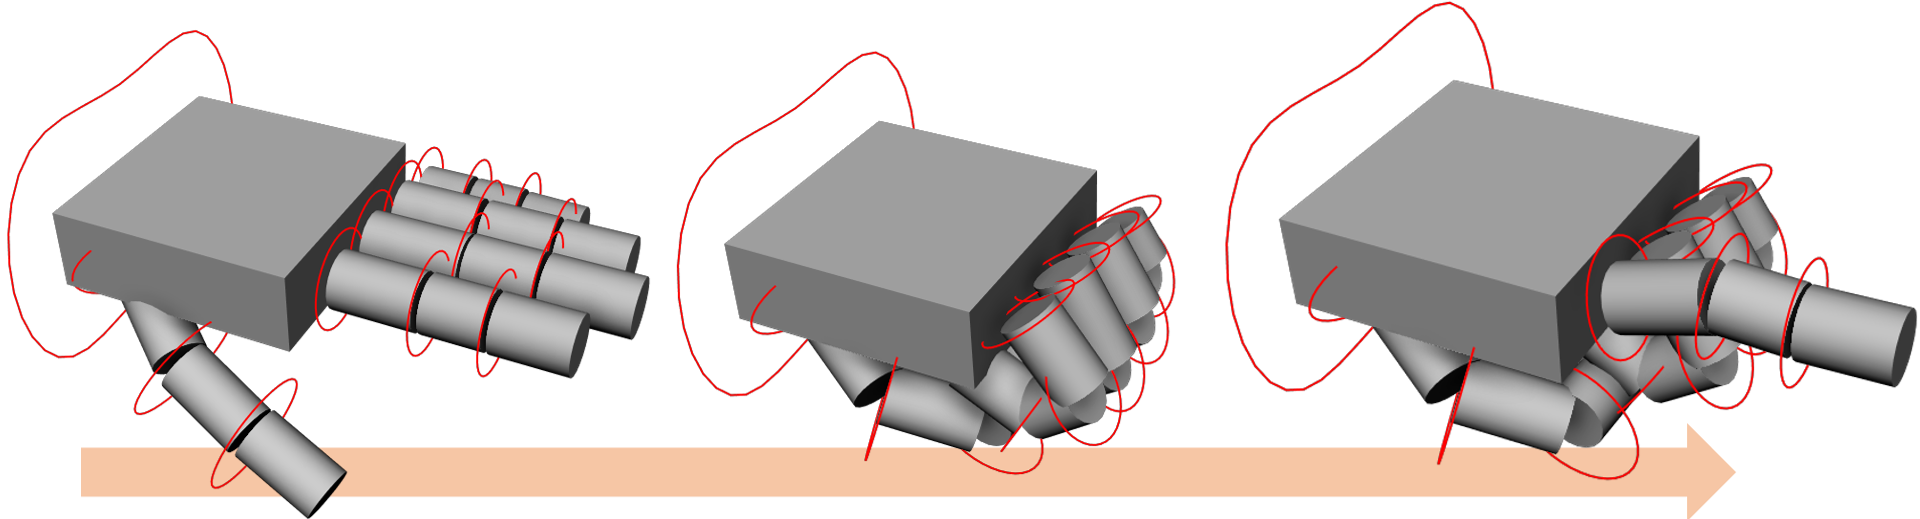
\includegraphics[width=3.0in]{images/handExample}
  \caption{Optimization results for the hand rig. The given motion is a sequence of the neutral, fist, and pointing hand pose.}
  \label{fig:handExample}
\end{figure}

\begin{figure}[!ht]
    \centering
    \begin{subfigure}[b]{0.48\textwidth}
        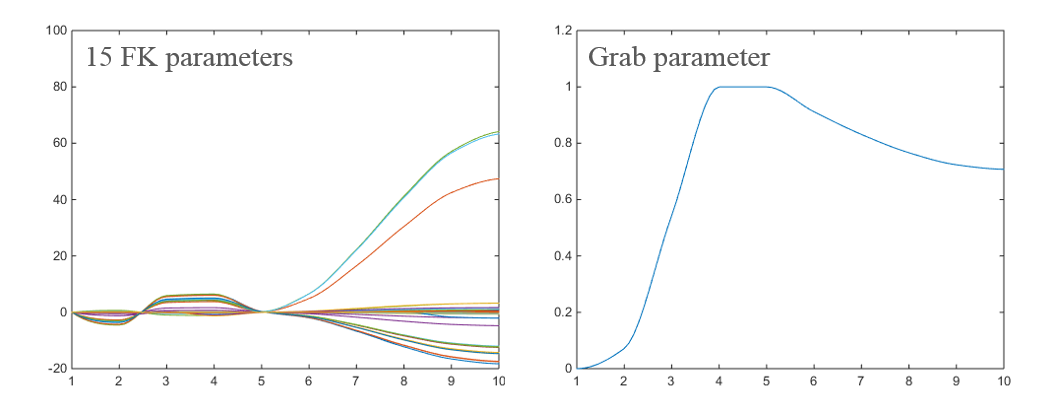
\includegraphics[width=\textwidth]{images/ls}
        \caption{L2 regularization}
        \label{fig:ls}
    \end{subfigure}
    %add desired spacing between images, e. g. ~, \quad, \qquad, \hfill etc. 
      %(or a blank line to force the subfigure onto a new line)
    \begin{subfigure}[b]{0.48\textwidth}
        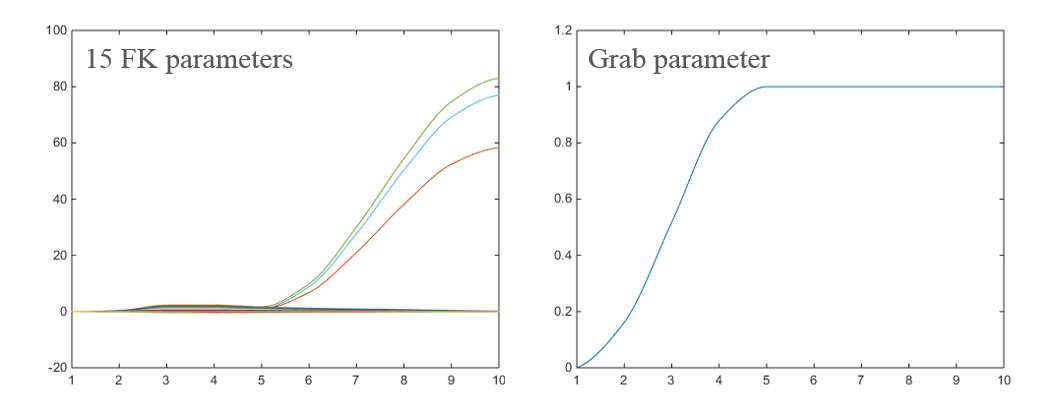
\includegraphics[width=\textwidth]{images/n1_good}
        \caption{L1 regularization ($\lambda = 0.001$)}
        \label{fig:reg_opt}
    \end{subfigure}
    
%    \begin{subfigure}[b]{0.45\textwidth}
%        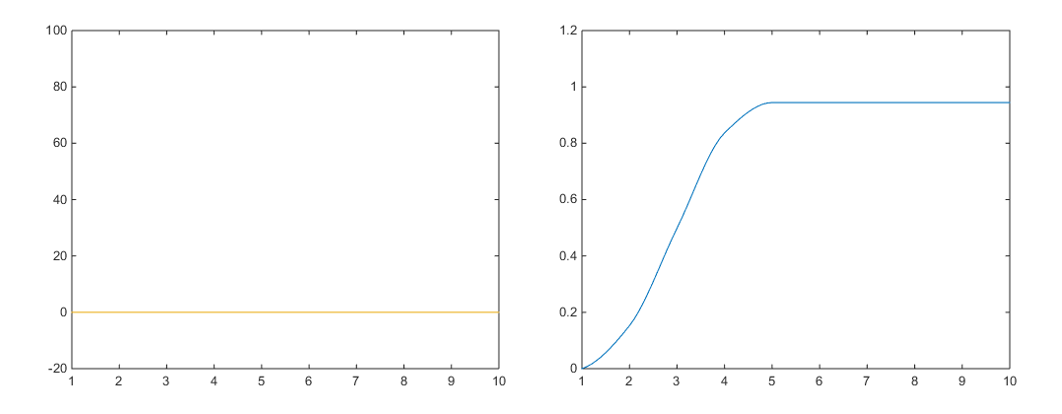
\includegraphics[width=\textwidth]{images/n1_big}
%        \caption{$\lambda = 1.0$}
%        \label{fig:reg_big}
%    \end{subfigure}
%    ~
%    \begin{subfigure}[b]{0.45\textwidth}
%        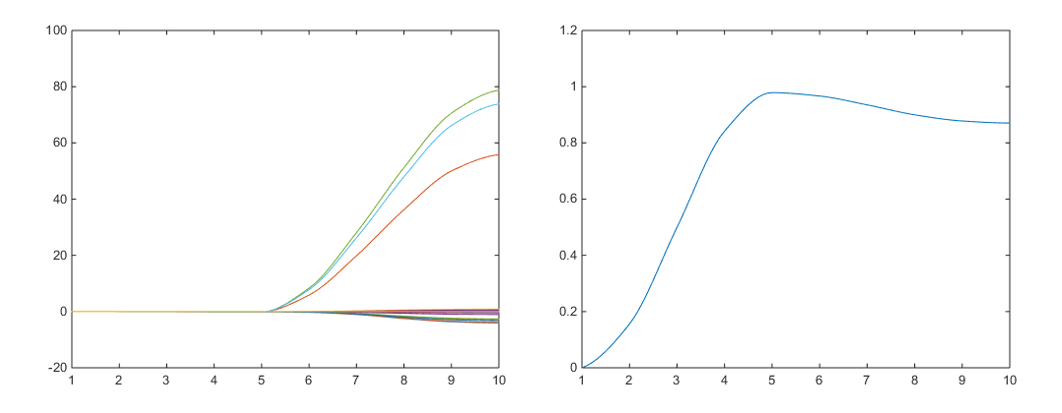
\includegraphics[width=\textwidth]{images/n1_small}
%        \caption{$\lambda = 0.0001$}
%        \label{fig:reg_small}
%    \end{subfigure}
    
    \caption{Comparison between optimization results of Figure~\ref{fig:handExample}.
    (a) FK parameters associated with all the fingers and grab parameter are used to generate pointing hand pose.
    (b) FK parameters of the index finger and grab parameter are used to generate the pointing hand pose.
    }
    \label{fig:reg}
\end{figure}

%\begin{figure*}[!ht]
%  \centering
%  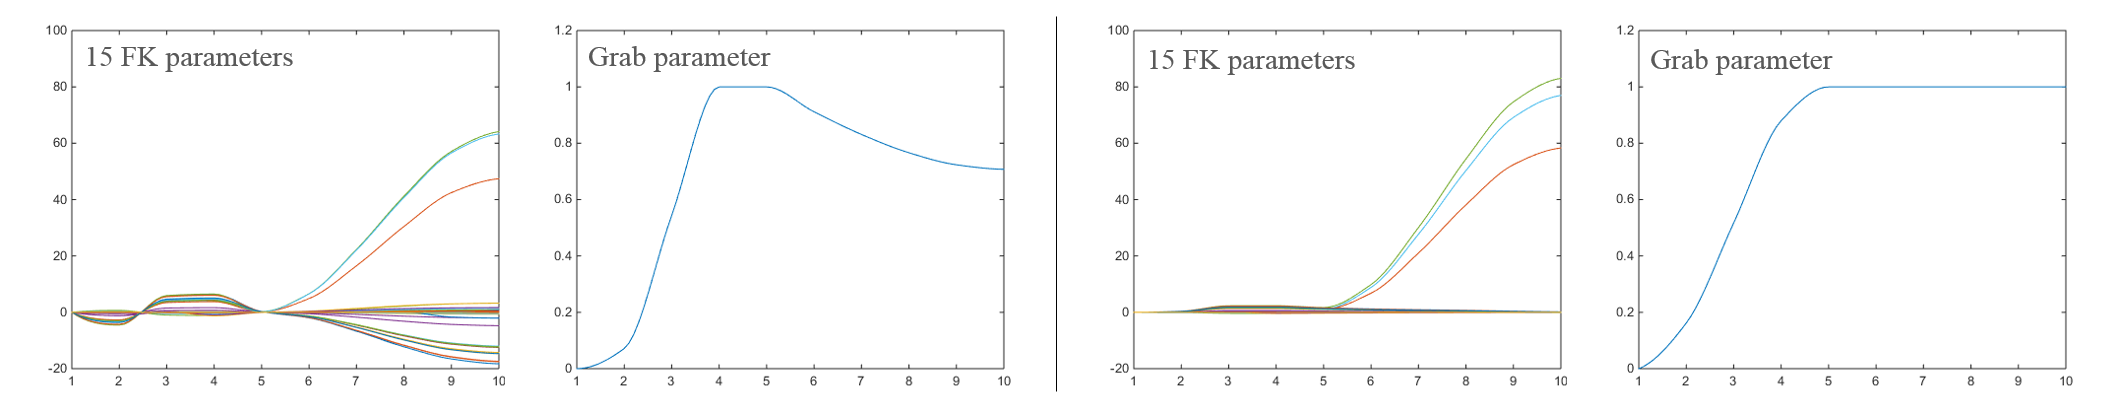
\includegraphics[width=0.95\textwidth]{images/reg}
%  \caption{Comparison between optimization results of Figure~\ref{fig:handExample}. ($\lambda = 0.001$) (left) L1 regularization (right) L2 regularization}
%  \label{fig:reg}
%\end{figure*}

%
%\begin{table}[ht]
%  \centering  
%  \begin{tabular}{|b|b b b|}
%    \hline
%     & Pose(a) & Pose(b) & Pose(c)\\
%    \hline
%    grab     & 1 & 1 & 0 \\
%    fingerFk & 0 & 6 & 15 \\
%    N(R)     & 1 & 7 & 15 \\
%    \hline
%  \end{tabular}
%  \caption{The number of activated rig parameters for various hand poses.}
%\end{table}

\textbf{Mapping results for various characters}
We applied the motion mapping to vaious target character rigs. Three different characters, which are rigged with FK only, FK+IK, and FK+IK+user defined parameters, respectively, are prepared for this purpose. Our method successfully maps the motion to various types of the rig space parameters as shown in Figure~\ref{fig:variousResult}. 
We also applied our method to a nonhuman character as shown in Figure~\ref{fig:dogResult}.
Figure~\ref{fig:squashResult} shows a result of our mapping of a stylized motion. As long as the rig space parameters can represent squash-and-stretches of the body parts, exaggerated source motion can be retargeted to a target character without any special treatment.
Although the pose representation with Lie group \SE{} is designed to work with rigid body motions, our method retargets stylized motion successfully, because the squash-and-strech motion can be represented by the translation of the skeletal segments.
This provides animation with great advantages of reusing high quality keyframed motions created by artists for different characters.

\begin{figure}[ht]
  \centering
  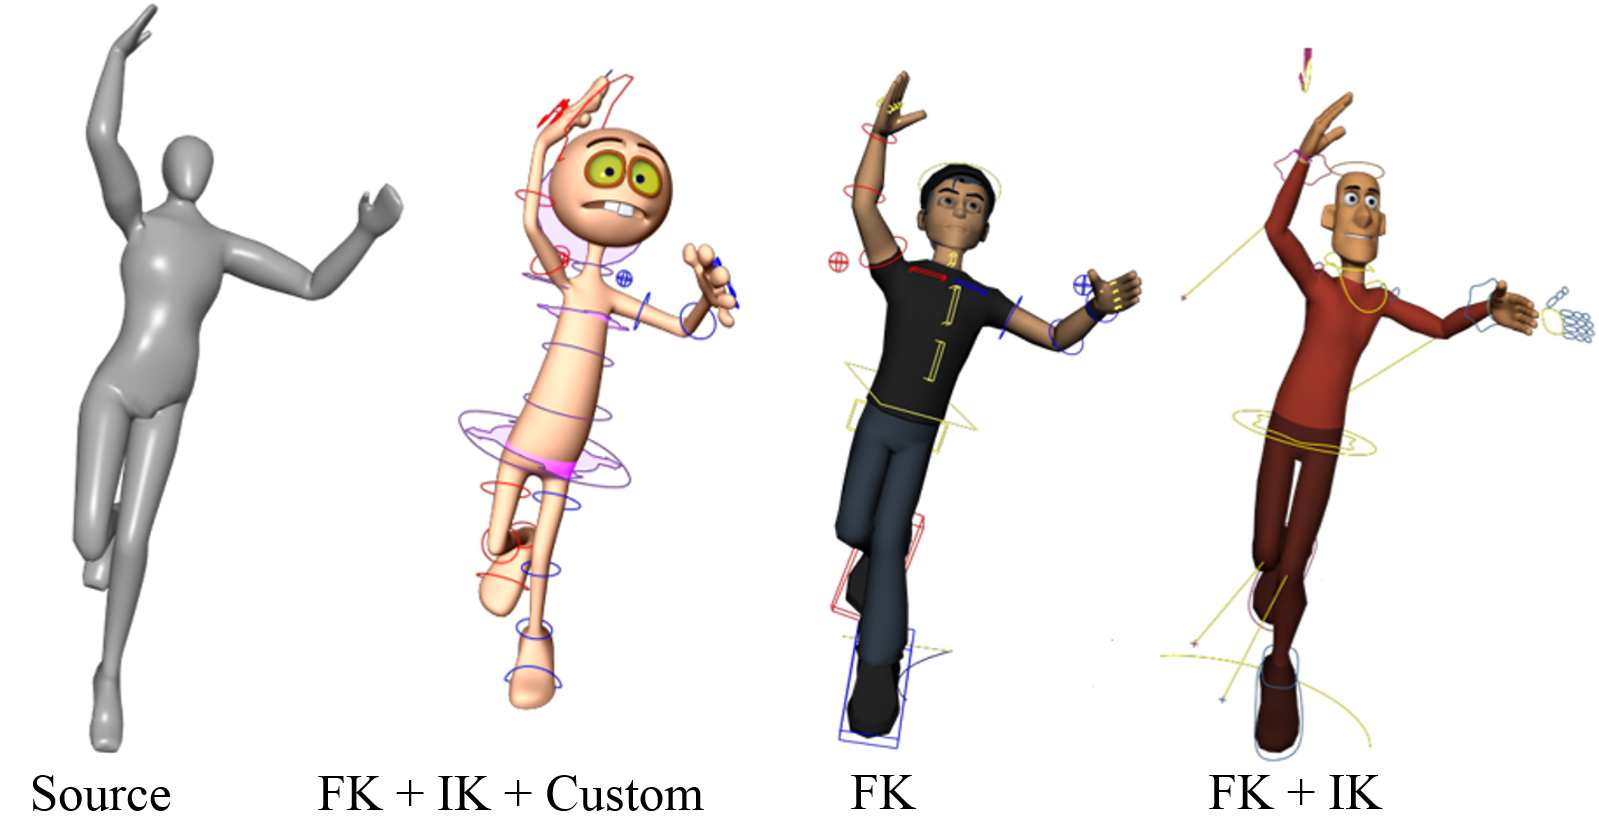
\includegraphics[width=1.0\linewidth]{images/various}
  \caption{Motion mapping results for three different characters.}
  \label{fig:variousResult}
\end{figure}

\begin{figure}[ht]
  \centering
  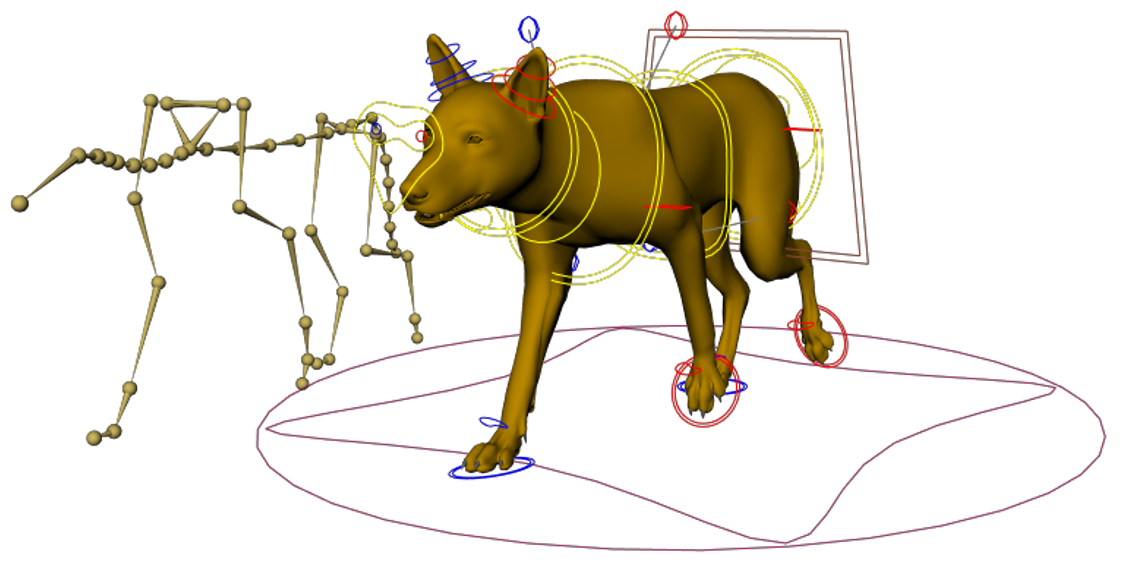
\includegraphics[width=.9\linewidth]{images/dogResult}
  \caption{Motion mapping results on quadruped character. }
  \label{fig:dogResult}
\end{figure}

\begin{figure}[ht]
  \centering
  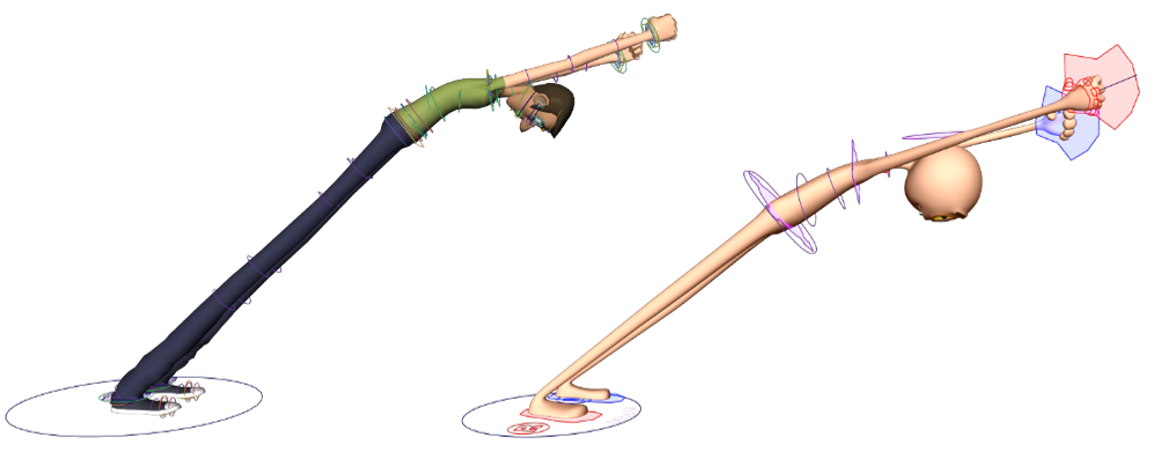
\includegraphics[width=.9\linewidth]{images/squashResult}
  \caption{Motion mapping result of stylized squash-and-stretch motion. }
  \label{fig:squashResult}
\end{figure}


\textbf{Editable optimization}
We provide the artist with editable optimization that is based on the relative skeletal segment constraint and the rig parameter constraint. Figure~\ref{fig:selfPenetration} shows a result of applying the relative skeletal constraint. Self-penetration is one of the most frequently occurring problems after a retargeting process, in general. Instead of performing the heavy mesh-level collision computation, we simply alleviate the problem with the use of relative constraints between the skeletal segments. 

\begin{figure}[ht]
  \centering
  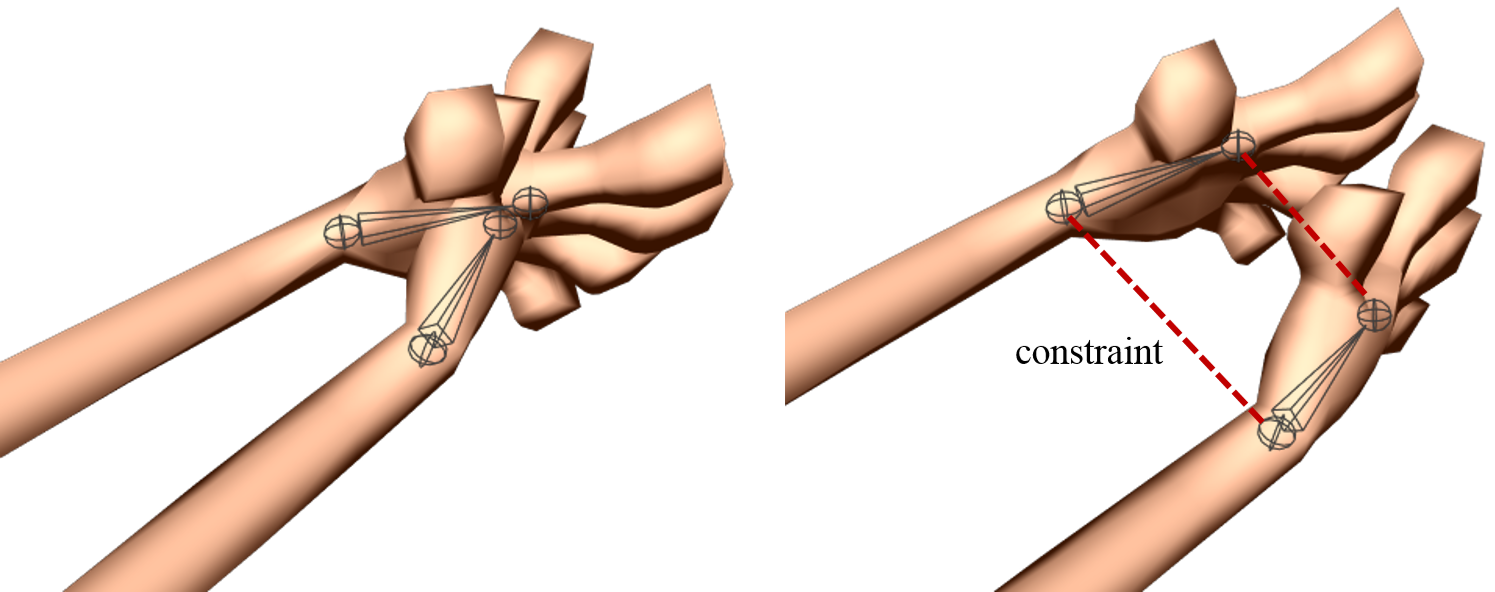
\includegraphics[width=.9\linewidth]{images/selfPenetration}
  \caption{(left) Self-penetration error after the initial optimization. (right) After the application of relative skeletal segment constraint given by artist.}
  \label{fig:selfPenetration}
\end{figure}

\textbf{Production pipeline evaluation}
Our method is suitable for the production pipeline, because the results produced by the rig space retargeting are something that artists would expect.
The subsequent editing process can be performed seamlessly.
To verify this, we applied our method to an animation project that exploits motion capture data as shown in Figure~\ref{fig:productionPipeline} which includes dynamic motions such as sword fighting and attacking of the dog.
For comparison, we additionaly measured working time required by 2 different methods to create the same animation: using keyframing and motion capture editing with commercial software, Autodesk MotionBuilder.
We performed the test with three different artists: one has 3 years of experiences, and the other two have 7 monthes of experiences.
As shown in Table~\ref{table:editing_evaluation}, our method required less time than keyframing or using commercial software. This verifies that our method can increase  efficiency in production.
Since artists are trained with using rigs in the existing animation pipeline, they also preferred our method that allows them to use the character rigs to edit the motion.
%All the animations were generated by three artists, one with 3 years experiences and the other two with 7 monthes of experiences.

%create a keyframe animation similiar to the motion capture scene. Then, we applied our method to the given motion capture data and the character rigs and presented to the artists for editing. Then, we measured the working time for both of the keyframing and the motion capture editing using our method.
%In addition, we measure the working time of motion capture editing with commercial software, Autodesk MotionBuilder$\textregistered$. 
%As shown in Table~\ref{table:editing_evaluation}, our method required less time than keyframing.


%\begin{table}[]
%\centering
%
%\begin{tabular}{c|c|c}
%\hline
%Artists                                                                                             & Method      & Working Time \\ \hline
%\multirow{3}{*}{\begin{tabular}[c]{@{}c@{}}One with 3-years of experience\\ \\ Two with 7-months of experience\end{tabular}} & Keyframing  & 10.7 Days    \\ \cline{2-3} 
%                                                                                                    & Mocap + MB   & 5 Days       \\ \cline{2-3} 
%                                                                                                    & Mocap + Ours & 3 Days       \\ \hline
%\end{tabular}
%\caption{Evaluation of our method to compared with keyframing and commercial software in the production pipeline environment.}
%\label{table:editing_evaluation}
%\end{table}
\begin{table}[!ht]
\centering
\begin{tabular}{ | c | c | }
  \hline
  Method & Average Working Time \\ \hline
  Mocap + Our Method & 3 Days \\ 
  Mocap + Commercial Software & 5 Days \\
  Keyframing & 10.7 Days \\
  \hline
\end{tabular}
\caption{Evaluation of our method compared with keyframing and using commercial software in the production pipeline environment. The result animations have 1140 frames.}
\label{table:editing_evaluation}
\end{table}

%\textbf{
%They create the dynamic motion of character efficiently from the motion capture editing with our method.
%Our method also required less amount of time to achieve the animation goal compared to the use of commercial software, because the artists are not expert with the software, and they prefer to use the character rigs to edit the motion because they already trained with the rigs in the exisiting animation pipeline. 
%}

\begin{figure}[!ht]
  \centering
  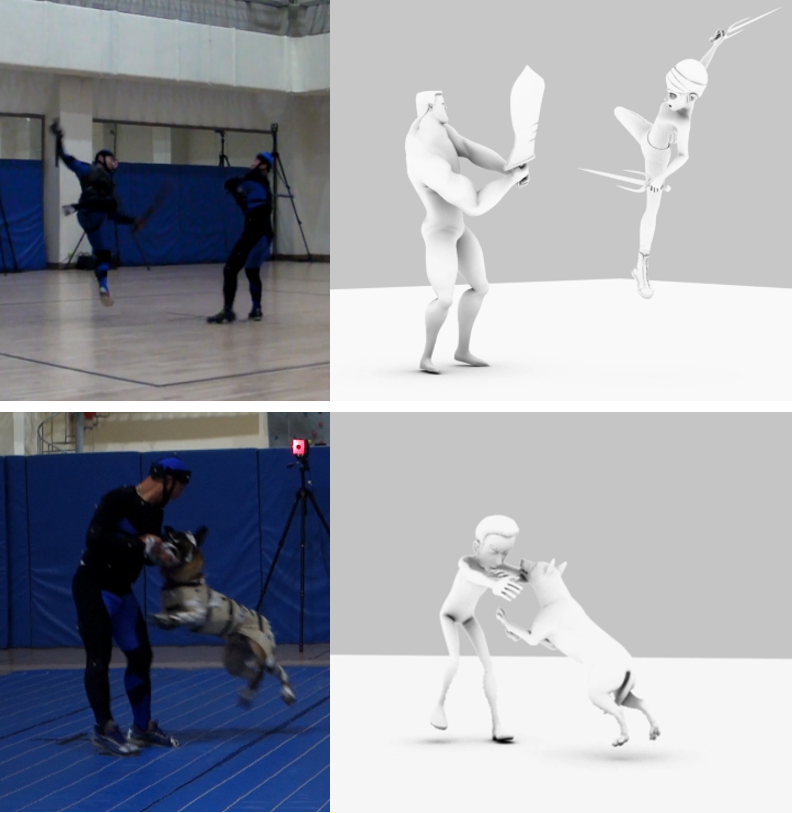
\includegraphics[width=1.0\linewidth]{images/production}
  \caption{Result of our method applied to the animation production pipeline. (Top) Snapshot of two character scene (Bottom) Snapshot of human and dog character scene}
  \label{fig:productionPipeline}
\end{figure}

%\begin{figure*}[ht]
%  \centering
%  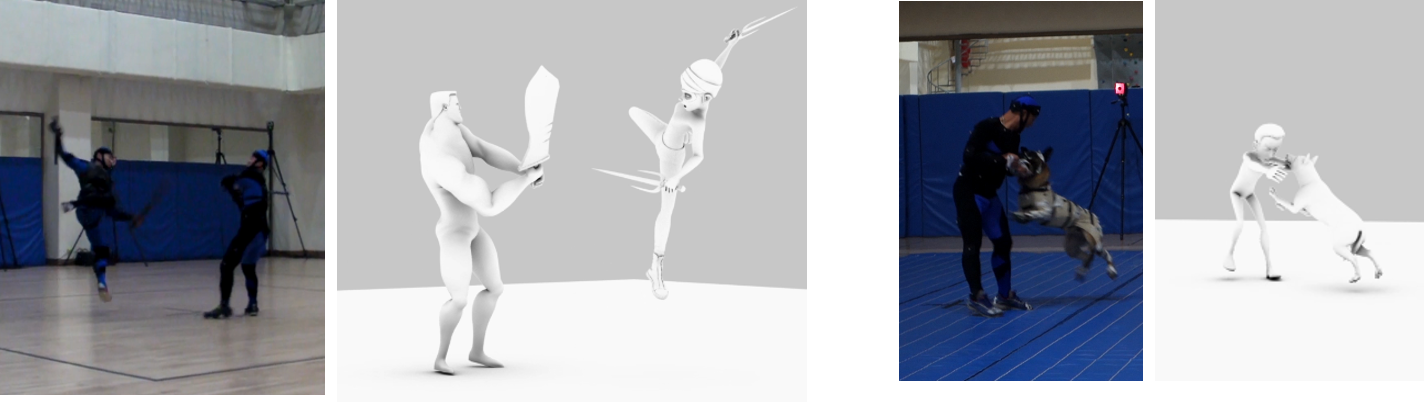
\includegraphics[width=.8\linewidth]{images/productionPipeline}
%  \caption{Result of our method applied to the animation production pipeline. (a) Snapshot of fighting two character scene (b) Snapshot of fighting human and dog character scene}
%  \label{fig:productionPipeline}
%\end{figure*}

%\begin{figure}[!ht]
%    \centering
%    \begin{subfigure}[b]{0.4\textwidth}
%        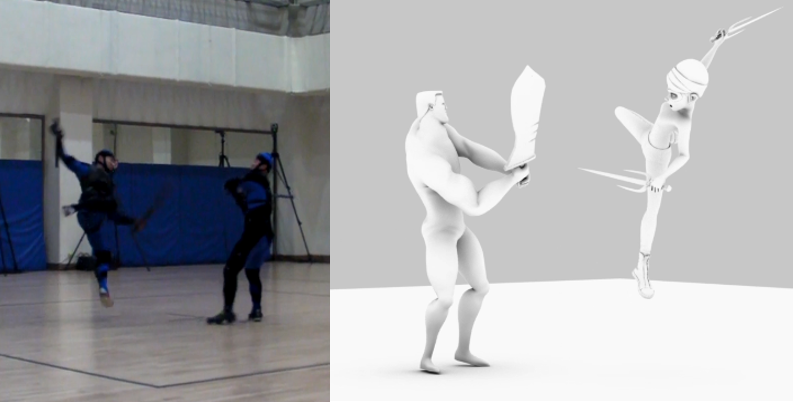
\includegraphics[width=\textwidth]{images/production1}
%        \caption{a}
%    \end{subfigure}
%    %add desired spacing between images, e. g. ~, \quad, \qquad, \hfill etc. 
%      %(or a blank line to force the subfigure onto a new line)
%    \begin{subfigure}[b]{0.4\textwidth}
%        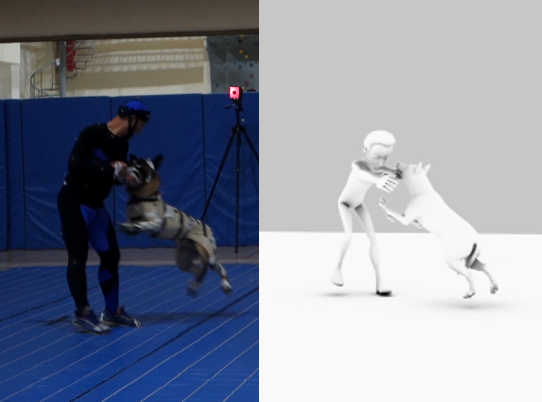
\includegraphics[width=\textwidth]{images/production2}
%        \caption{b}
%    \end{subfigure}
%    
%    \caption{Production Example
%    }
%    \label{fig:productionPipeline}
%\end{figure}

%\begin{table*}[ht]
%  \centering
%  \caption{An average error of different skeleton representation methods.}
%  \begin{tabular}{|b|b b b b b|}
%    \hline
%    Character & Joint Position & Joint Angle & Only Hierarchy & Only Global & Proposed \\
%    \hline
%    character A & & & & &\\
%    character B & & & & & \\
%    character C & & & & & \\
%    character D & & & & & \\
%    \hline
%  \end{tabular}
%\end{table*}